%!TEX TS-program = xelatex
% Защита магистерской диссертации — НИУ ВШЭ
% 20 слайдов, ~20 минут

\documentclass[aspectratio=169,9pt]{beamer}

% Включаем нумерацию слайдов
\setbeamertemplate{footline}[frame number]

\newbool{russian}
\booltrue{russian}
\usepackage{HSE-theme/beamerthemeHSE}

%%% Язык и шрифты
\usepackage[english,russian]{babel}
\usepackage[no-math]{fontspec}
  \setsansfont{HSESans-Regular}[
    Path = fonts/,
    Extension = .otf,
    BoldFont = HSESans-Bold,
    ItalicFont = HSESans-Italic,
    BoldItalicFont = HSESans-Bold,
    SemiBoldFont = HSESans-SemiBold,
  ]
  \setmonofont{Courier New}
\usepackage{mathspec}
  \setmathsfont(Digits,Latin,Greek)[
    Path = fonts/, Extension = .otf,
    Numbers={Lining,Proportional}
  ]{HSESans-Regular}
  \setmathrm[Path = fonts/, Extension = .otf,
    Numbers={Lining,Proportional}
  ]{HSESans-Regular}
\uselanguage{russian}
\languagepath{russian}

%%% Доп. пакеты
\usepackage{booktabs}
\usepackage{tabularx}
\usepackage{tikz}
\usetikzlibrary{arrows.meta, positioning, shapes.geometric, fit, backgrounds}
\usepackage{xcolor}
\usepackage{amssymb}

%%% Псевдокод (как в тексте диссертации) и подсветка кода
\usepackage{float}
\usepackage[ruled,vlined,linesnumbered]{algorithm2e}
\DontPrintSemicolon
\usepackage{listings}
\definecolor{lstkw}{HTML}{0B5FA5}
\definecolor{lststr}{HTML}{1A7F37}
\definecolor{lstcom}{HTML}{8A8A8A}
\definecolor{lstbg}{HTML}{F4F6FA}
\lstdefinestyle{py}{
  language=Python,
  basicstyle=\ttfamily\footnotesize,
  keywordstyle=\color{lstkw}\bfseries,
  stringstyle=\color{lststr},
  commentstyle=\color{lstcom}\itshape,
  showstringspaces=false,
  breaklines=true,
  columns=fullflexible,
  keepspaces=true,
  frame=single,
  rulecolor=\color{gray!35},
  backgroundcolor=\color{lstbg},
  framesep=6pt,
  xleftmargin=10pt,
  xrightmargin=4pt,
  aboveskip=2pt,
  belowskip=2pt,
}

\graphicspath{{images/}{../thesis/figures/}}

%%% Плейсхолдер для будущих авторских схем
\newcommand{\schemaTODO}[3]{%
  \begin{tikzpicture}
    \draw[dashed, very thick, color=gray!70, fill=gray!5]
      (0,0) rectangle (#1,#2);
    \node[align=center, font=\small, text=gray!80]
      at (#1/2, #2/2) {\textbf{TODO}\\#3};
  \end{tikzpicture}}

%%% Мета
\title[Поиск кандидатов на GPU]{Методы поиска кандидатов на графических ускорителях в рекомендательных системах}
\author[Нигматуллин Р.\,М.]{Нигматуллин Роман Максимович \\ \smallskip \scriptsize Научный руководитель: Хрыльченко Кирилл Ярославович}
\institute{Факультет компьютерных наук\\ОП "Современные компьютерные науки"}
\date{Москва, 2026}

% ═════════════════════════════════════════════════════════════════════════════
\begin{document}

% ── 1. ТИТУЛ ─────────────────────────────────────────────────────────────────
\frame[plain]{\titlepage}

% ── 2. АКТУАЛЬНОСТЬ ──────────────────────────────────────────────────────────
\begin{frame}
\frametitle{Актуальность и контекст}

\begin{columns}[T]
\column{0.58\textwidth}
  \textbf{Двухстадийная архитектура} рекомендательной системы:
  поиск кандидатов сужает каталог из $10^6$--$10^9$ объектов до $10^2$--$10^3$
  для последующего ранжирования.

  \vspace{0.3em}
  \textbf{Жёсткие требования к этапу поиска:}
  \begin{itemize}\small
    \item \alert{Скорость} --- от единиц до сотен мс на запрос
    \item \alert{Полнота} --- $\mathrm{Recall@}K$ определяет потолок качества всего конвейера
    \item \alert{Фильтрация} по атрибутам объектов (жанр, язык, регион, лицензия)
    \item \alert{Память} --- каталоги до $10^9$, рост размерности эмбеддингов
  \end{itemize}

  \vspace{0.3em}
  \textbf{Тенденция:} переход от статических ANN-индексов к
  поиску на основе модели.

\column{0.40\textwidth}
  \centering
  \begin{tikzpicture}[
    node distance=0.42cm,
    box/.style={draw, rounded corners=3pt, fill=blue!6,
                text width=3.3cm, align=center,
                font=\small, minimum height=0.6cm},
    opt/.style={draw, dashed, rounded corners=3pt, fill=blue!3,
                text width=3.3cm, align=center,
                font=\small, minimum height=0.6cm},
    arr/.style={-Stealth, thick, color=HSEblue}
  ]
    \node[box] (q)  {эмбеддинг запроса};
    \node[opt, below=of q] (f1) {префильтрация (опц.)};
    \node[box, below=of f1] (r)  {поиск (1-й уровень)};
    \node[opt, below=of r] (f2) {пост-фильтрация (опц.)};
    \node[box, below=of f2] (k)  {top-$K$ результатов};
    \draw[arr] (q)--(f1);
    \draw[arr] (f1)--(r);
    \draw[arr] (r)--(f2);
    \draw[arr] (f2)--(k);
  \end{tikzpicture}
\end{columns}
\end{frame}

% ── 3. ОБЗОР ПРЕДМЕТНОЙ ОБЛАСТИ ──────────────────────────────────────────────
\begin{frame}
\frametitle{Обзор: методы векторного поиска}

\begin{itemize}
  \item \textbf{Квантизация и инвертированные индексы (IVF):} Product / Scalar Quantization, ScaNN.
  \item \textbf{Графовые алгоритмы:} HNSW, DiskANN, NVIDIA CAGRA (GPU), SONG.
  \item \textbf{Векторные СУБД на GPU:} Milvus. 
        \alert{Недостатки:} низкоуровневый код (C++), вызывают разрывы вычислительного графа PyTorch, отсутствие гибкой атрибутной фильтрации прямо на GPU.
\end{itemize}

\vspace{0.5em}
\begin{block}{Поиск на основе модели (LiNR, LinkedIn 2024)}
  Поиск кандидатов выражен как единый слой \texttt{nn.Module} (индекс + вычисления). Оценки сходства (скоры) вычисляются на лету с одновременной фильтрацией внутри графа нейросети.
  
  \alert{Проблема:} проприетарный код, алгоритмы V1--V3 недоступны для открытого тестирования и использования, что и мотивирует создание нашего решения.
\end{block}
\end{frame}

% ── 4. ЦЕЛЬ И РЕШАЕМЫЕ ПРОБЛЕМЫ ──────────────────────────────────────────────
\begin{frame}
\frametitle{Цель работы и её вклад}

\textbf{Цель.} Создать открытый фреймворк \texttt{torchretrieve} на PyTorch + Triton для поиска кандидатов на GPU с поддержкой атрибутной фильтрации, который легко встраивается в граф вычислений модели и совместим с \texttt{torch.compile}.

\vspace{0.8em}
\textbf{Решаемые проблемы и вклад:}
\begin{itemize}
  \item \textbf{Проблема закрытости кода:} Воспроизведены индустриальные алгоритмы LiNR V1--V3 под единым открытым API.
  \item \textbf{Проблема нехватки релевантных кандидатов (liquidity):} Реализована фильтрация прямо в процессе поиска, предотвращающая вытеснение релевантных объектов.
  \item \textbf{Высокое потребление памяти:} Предложен новый INT8-вариант \textbf{LiNR V4}, снижающий объем индекса в два раза при $\ge 95\%$ полноты.
  \item \textbf{Скорость работы:} Разработан авторский алгоритм \textbf{QuantizedIVF} (IVF + INT8 + фильтр Блума), работающий в одном Triton-ядре (ускорение до ${\approx}9\times$).
\end{itemize}
\end{frame}

% ── 5. ПОСТАНОВКА ЗАДАЧИ ─────────────────────────────────────────────────────
\begin{frame}
\frametitle{Формальная постановка задачи}

\begin{columns}[T]
\column{0.54\textwidth}
  Пусть $X \in \mathbb{R}^{N \times D}$ --- каталог из $N$ объектов, $Q \in \mathbb{R}^{B \times D}$ --- батч запросов.
  Атрибутный фильтр задает допустимые объекты с помощью бинарной маски $M\in\{0,1\}^{B\times N}$.

  \vspace{0.5em}
  \textbf{Задача:} для каждого запроса $q_i$ найти:
  \[
    I_i \;=\; \arg\mathrm{top}\text{-}K \;\bigl\{\, q_i^\top x_j \;\bigm|\; M[i,j] = 1 \,\bigr\}.
  \]

  \vspace{0.5em}
  \textbf{Ограничения системы:}
  \begin{itemize}\small
    \item требования к времени ответа $t_\mathrm{med}$;
    \item пиковое потребление памяти GPU;
    \item интеграция в граф PyTorch без разрывов.
  \end{itemize}

\column{0.44\textwidth}
  \begin{block}{Методология оценки}
    \textbf{Базовый метод:} точный векторный поиск (KNN) полным перебором с маскированием.

    \vspace{0.5em}
    Все приближённые алгоритмы сравниваются по скорости и полноте ($\mathrm{Recall@}K$) относительно этого базового метода.
  \end{block}
\end{columns}
\end{frame}

% ── 6. LiNR V1 и V2 ────────────────────────────────────────────────────────────
\begin{frame}
\frametitle{LiNR V1 и V2 --- точный поиск с фильтрацией}

\begin{columns}[T]
\column{0.42\textwidth}
  {\footnotesize
  \textbf{V1 --- постфильтрация}
  \begin{itemize}
    \item Считаем все скоры сходства.
    \item Заменяем отфильтрованные на $-\infty$.
  \end{itemize}

  \vspace{0.6em}
  \textbf{V2 --- префильтрация}
  \begin{itemize}
    \item Сначала отбираем прошедшие фильтр объекты.
    \item Считаем скоры сходства только для них.
  \end{itemize}
  \par}
  \vspace{1em}
  \footnotesize\textit{Алгоритмы из статьи LiNR\\
  (Borisyuk et al., LinkedIn, 2024).}

\column{0.56\textwidth}
  \centering
  \begin{tikzpicture}[
    font=\footnotesize,
    box/.style={draw, rounded corners=3pt, fill=blue!6, align=center,
                inner sep=3pt, minimum height=0.6cm, text width=2.5cm},
    hi/.style={draw, rounded corners=3pt, fill=HSEblue!16, align=center,
               inner sep=3pt, minimum height=0.6cm, text width=2.5cm,
               font=\footnotesize\bfseries},
    arr/.style={-Stealth, very thick, color=HSEblue},
    hdr/.style={font=\footnotesize\bfseries, text=HSEblue}
  ]
    \def\xa{1.75}\def\xb{5.25}
    \node[hdr] at (\xa,1.0) {V1 --- постфильтр};
    \node[hdr] at (\xb,1.0) {V2 --- префильтр};
    % ── V1 column ──
    \node[box] (a1) at (\xa,0)     {Запрос};
    \node[hi]  (b1) at (\xa,-1.35) {Расчёт всех скоров\\[-1pt]{\scriptsize\textcolor{HSEorange}{весь каталог}}};
    \node[box] (c1) at (\xa,-2.7)  {Маскирование};
    \node[box] (d1) at (\xa,-4.05) {Отбор top-$K$};
    \draw[arr] (a1)--(b1); \draw[arr] (b1)--(c1); \draw[arr] (c1)--(d1);
    % ── V2 column ──
    \node[box] (a2) at (\xb,0)     {Запрос};
    \node[box] (b2) at (\xb,-1.35) {Отбор по фильтру};
    \node[hi]  (c2) at (\xb,-2.7)  {Расчёт для отфильтрованных\\[-1pt]{\scriptsize\textcolor{HSEorange}{прошедшие фильтр}}};
    \node[box] (d2) at (\xb,-4.05) {Отбор top-$K$\\[-1pt]{\scriptsize\textcolor{HSEorange}{+ ремап индексов}}};
    \draw[arr] (a2)--(b2); \draw[arr] (b2)--(c2); \draw[arr] (c2)--(d2);
  \end{tikzpicture}
\end{columns}
\end{frame}

% ── 7. LiNR V3 ───────────────────────────────────────────────────────────────
\begin{frame}
\frametitle{LiNR V3 --- Sign-OPORP + расстояние Хэмминга}

\begin{columns}[T]
\column{0.42\textwidth}
  {\footnotesize
  \textbf{Двухэтапный поиск} (Sign-OPORP, Li 2023)
  \begin{itemize}
    \item \textbf{Сжатие:} эмбеддинги бинаризуются до 1 бита на размерность.
    \item \textbf{Грубый отбор:} фильтрация + быстрый поиск по расстоянию Хэмминга.
    \item \textbf{Точный пересчёт:} точные скоры (rescore) для пула кандидатов.
  \end{itemize}
  \par}
  \vspace{1em}
  \footnotesize $W=\lceil D/64\rceil$; $P_c$ --- размер пула кандидатов для точного пересчёта.

\column{0.56\textwidth}
  \centering
  \begin{tikzpicture}[
    font=\footnotesize,
    box/.style={draw, rounded corners=3pt, fill=blue!6, align=center,
                inner sep=3pt, minimum height=0.5cm, text width=2.5cm},
    hi/.style={draw, rounded corners=3pt, fill=HSEblue!16, align=center,
               inner sep=3pt, minimum height=0.5cm, text width=2.5cm,
               font=\footnotesize\bfseries},
    off/.style={draw, dashed, rounded corners=3pt, fill=blue!3, align=center,
                inner sep=3pt, minimum height=0.5cm, text width=2.0cm},
    arr/.style={-Stealth, very thick, color=HSEblue},
    arrd/.style={-Stealth, thick, dashed, color=HSEblue}
  ]
    \def\xo{1.45}\def\xn{5.1}
    % ── Online column (right) ──
    \node[box] (q)    at (\xn,0.2)   {Запрос};
    \node[box] (so)   at (\xn,-1.0)  {Sign-OPORP};
    \node[hi]  (ham)  at (\xn,-2.2)  {Грубый отбор\\(по Хэммингу)};
    \node[box] (resc) at (\xn,-3.4)  {Точный пересчёт\\(rescore)};
    \node[box] (topk) at (\xn,-4.6)  {Отбор top-$K$};
    \draw[arr] (q)--(so); \draw[arr] (so)--(ham);
    \draw[arr] (ham)--(resc); \draw[arr] (resc)--(topk);
    % ── Offline column (left, dashed) ──
    \node[off] (cat) at (\xo,-0.4) {Каталог};
    \node[off] (so2) at (\xo,-1.6) {Sign-OPORP};
    \node[off] (bx)  at (\xo,-2.8) {Битовый индекс};
    \draw[arrd] (cat)--(so2); \draw[arrd] (so2)--(bx);
    \draw[arrd] (bx) -- (ham.west);
    \begin{scope}[on background layer]
      \node[draw=gray!55, dashed, rounded corners=4pt, fill=gray!4,
            fit=(cat)(so2)(bx), inner sep=5pt] (offbox) {};
    \end{scope}
    \node[font=\scriptsize, text=gray!70, anchor=south] at (offbox.north) {offline};
  \end{tikzpicture}
\end{columns}
\end{frame}

% ── 8. LiNR V4 (вклад работы) ───────────────────────────────────────────────
\begin{frame}
\frametitle{LiNR V4 --- INT8-квантизация (вклад работы)}

\begin{columns}[T]
\column{0.42\textwidth}
  {\footnotesize
  \textbf{Модификация V1 с INT8-квантизацией}
  \begin{itemize}
    \item Скалярная INT8-квантизация каталога с \textbf{общим масштабом} (scale).
    \item Поиск top-$K$ осуществляется сразу в формате INT32.
    \item Деквантизация в числа с плавающей точкой только для итогового ответа.
  \end{itemize}
  \par}
  \vspace{1em}
  \footnotesize Общий масштаб $s_X$ позволяет находить top-$K$ без деквантизации
  всех скоров.

\column{0.56\textwidth}
  \centering
  \begin{tikzpicture}[
    font=\footnotesize,
    box/.style={draw, rounded corners=3pt, fill=blue!6, align=center,
                inner sep=3pt, minimum height=0.5cm, text width=2.5cm},
    hi/.style={draw, rounded corners=3pt, fill=HSEblue!16, align=center,
               inner sep=3pt, minimum height=0.5cm, text width=2.5cm,
               font=\footnotesize\bfseries},
    off/.style={draw, dashed, rounded corners=3pt, fill=blue!3, align=center,
                inner sep=3pt, minimum height=0.5cm, text width=2.0cm},
    arr/.style={-Stealth, very thick, color=HSEblue},
    arrd/.style={-Stealth, thick, dashed, color=HSEblue}
  ]
    \def\xo{1.45}\def\xn{5.1}
    % ── Online column (right) ──
    \node[box] (q)    at (\xn,0.2)   {Запрос};
    \node[box] (qq)   at (\xn,-1.0)  {INT8-квантизация};
    \node[hi]  (gemm) at (\xn,-2.2)  {INT8-умножение\\[-1pt]{\scriptsize\textcolor{HSEorange}{общий масштаб}}};
    \node[box] (mask) at (\xn,-3.6)  {Маскирование};
    \node[box] (topk) at (\xn,-4.8)  {Отбор top-$K$};
    \draw[arr] (q)--(qq); \draw[arr] (qq)--(gemm);
    \draw[arr] (gemm)--(mask); \draw[arr] (mask)--(topk);
    % ── Offline column (left, dashed) ──
    \node[off] (cat) at (\xo,-0.4) {Каталог};
    \node[off] (oq)  at (\xo,-1.6) {INT8-квантизация};
    \node[off] (xi)  at (\xo,-2.8) {Квант. индекс};
    \draw[arrd] (cat)--(oq); \draw[arrd] (oq)--(xi);
    \draw[arrd] (xi) -- (gemm.west);
    \begin{scope}[on background layer]
      \node[draw=gray!55, dashed, rounded corners=4pt, fill=gray!4,
            fit=(cat)(oq)(xi), inner sep=5pt] (offbox) {};
    \end{scope}
    \node[font=\scriptsize, text=gray!70, anchor=south] at (offbox.north) {offline};
  \end{tikzpicture}
\end{columns}
\end{frame}

% ── 9. QuantizedIVF (вклад работы) ──────────────────────────────────────────
\begin{frame}
\frametitle{QuantizedIVF --- авторский алгоритм с фильтрацией}

\begin{columns}[T]
\column{0.42\textwidth}
  \textbf{Triton-ядро со встроенным фильтром}
  \begin{itemize}
    \item \textbf{Кластеризация:} отбор ближайших кластеров к запросу.
    \item \textbf{Фильтрация:} внутри кластеров отсекаются нерелевантные объекты.
    \item \textbf{INT8-поиск:} для прошедших фильтрацию кандидатов скоры вычисляются в INT8.
  \end{itemize}

  \vspace{0.8em}
  {\footnotesize
  \textbf{Фаза Filter --- два варианта \texttt{FilterModule} (доступны любому алгоритму):}
  \textbf{ExactAttributeFilter} --- точная проверка по значениям, без ложных
  срабатываний; подходит при небольшом числе атрибутов и необходимости
  гарантированной полноты.
  \textbf{BloomFilter} --- компактные 1024-битные сигнатуры и быстрый побитовый
  AND; оптимален для экономии памяти при большом числе атрибутов,
  допуская ложноположительные срабатывания (считаются нерелевантными).
  \par}

\column{0.56\textwidth}
  \centering
  \begin{tikzpicture}[
    font=\footnotesize,
    box/.style={draw, rounded corners=3pt, fill=blue!6, align=center,
                inner sep=3pt, minimum height=0.5cm, text width=2.5cm},
    sub/.style={draw, rounded corners=3pt, fill=blue!6, align=center,
                inner sep=2.5pt, minimum height=0.5cm, text width=1.45cm},
    hi/.style={draw, rounded corners=3pt, fill=HSEblue!16, align=center,
               inner sep=3pt, minimum height=0.5cm, text width=2.5cm,
               font=\footnotesize\bfseries},
    off/.style={draw, dashed, rounded corners=3pt, fill=blue!3, align=center,
                inner sep=3pt, minimum height=0.5cm, text width=1.9cm},
    arr/.style={-Stealth, very thick, color=HSEblue},
    arrd/.style={-Stealth, thick, dashed, color=HSEblue},
    note/.style={font=\scriptsize, text=HSEorange, align=center},
    lbl/.style={font=\footnotesize\bfseries, text=HSEblue}
  ]
    % ── Kernel column (vertical 3-phase flow) ──
    \node[box] (p)   at (5.0,0.3)   {Отбор кластеров};
    \node[sub] (fb)  at (4.05,-1.2) {Bloom-\\фильтр};
    \node[sub] (fa)  at (5.95,-1.2) {Точный\\фильтр};
    \node[hi]  (s)   at (5.0,-2.6)  {INT8-оценка};
    \node[box] (out) at (5.0,-3.85) {Отбор top-$K$};
    \draw[arr] (p)--(fb); \draw[arr] (p)--(fa);
    \draw[arr] (fb)--(s); \draw[arr] (fa)--(s);
    \draw[arr] (s)--(out);
    % ── Offline (left, parallel prep) ──
    \node[off] (o1) at (1.3,0.3)   {k-means++};
    \node[off] (o3) at (1.3,-1.2)  {Bloom-кодирование};
    \node[off] (o2) at (1.3,-2.6)  {INT8-квантизация};
    \draw[arrd] (o1) -- (p.west);
    \draw[arrd] (o3) -- (fb.west);
    \draw[arrd] (o2) -- (s.west);
    % ── fit boxes (background) ──
    \begin{scope}[on background layer]
      \node[draw=HSEblue, thick, rounded corners=4pt, fill=HSEblue!4,
            fit=(p)(fb)(fa)(s)(out), inner sep=7pt] (kern) {};
      \node[draw=gray!55, dashed, rounded corners=4pt, fill=gray!4,
            fit=(o1)(o3)(o2), inner sep=5pt] (offbox) {};
    \end{scope}
    \node[lbl, anchor=south] at (kern.north) {Triton-ядро};
    \node[font=\scriptsize, text=gray!70, anchor=south] at (offbox.north) {offline};
    \node[note, anchor=north] at (kern.south) {одно ядро, без разрывов графа};
  \end{tikzpicture}
\end{columns}
\end{frame}

% ── 10. АРХИТЕКТУРА И API ────────────────────────────────────────────────────
\begin{frame}
\frametitle{Архитектура фреймворка и API}

\begin{columns}[T]
\column{0.42\textwidth}
  \textbf{Архитектурные принципы}
  \begin{itemize}\footnotesize
    \item Каждый алгоритм --- стандартный \texttt{nn.Module}
    \item Единый интерфейс \texttt{FilterModule} для атрибутов
    \item Два бэкенда: оптимизированный Triton + эталонный PyTorch
    \item Ядра регистрируются через \texttt{@torch.library.triton\_op}
    \item Отсутствие разрывов вычислительного графа (graph breaks)
    \item Предварительная (offline) автонастройка параметров ядер
  \end{itemize}

\column{0.56\textwidth}
  \centering
  \begin{tikzpicture}[
    font=\footnotesize,
    box/.style={draw, rounded corners=3pt, fill=blue!6, align=center,
                inner sep=3pt, minimum height=0.5cm, text width=1.95cm},
    sub/.style={draw, rounded corners=3pt, fill=HSEblue!14, align=center,
                inner sep=2.5pt, minimum height=0.42cm, text width=1.95cm},
    off/.style={draw, dashed, rounded corners=3pt, fill=blue!3, align=center,
                inner sep=3pt, minimum height=0.5cm, text width=1.85cm},
    arr/.style={-Stealth, very thick, color=HSEblue},
    arrd/.style={-Stealth, thick, dashed, color=HSEblue},
    note/.style={font=\scriptsize, text=HSEorange, align=center},
    lbl/.style={font=\scriptsize, text=HSEblue}
  ]
    \def\cx{4.5}
    % ── Online path inside compile block ──
    \node[box] (in)   at (\cx,0.4)    {Запрос + атрибуты};
    \node[box] (filt) at (3.2,-0.95)  {FilterModule};
    \node[box] (enc)  at (5.8,-0.95)  {Энкодер запроса};
    \node[box, fill=HSEblue!14, font=\footnotesize\bfseries]
               (retr) at (\cx,-2.3)   {RetrieverModule};
    \node[box] (topk) at (\cx,-3.7)   {Отбор top-$K$};
    \draw[arr] (in)--(filt);
    \draw[arr] (in)--(enc);
    \draw[arr] (filt) -- (retr.north west) node[lbl, pos=0.2, left=-1pt] {mask};
    \draw[arr] (enc)  -- (retr.north east) node[lbl, pos=0.2, right=-1pt] {$q$};
    \draw[arr] (retr)--(topk);
    % ── Offline blocks (left, outside) ──
    \node[off] (ria) at (0.45,-0.95) {register\_index\\(атрибуты)};
    \node[off] (rie) at (0.45,-2.35) {register\_index\\(эмбеддинги)};
    \node[off] (auto) at (0.45,-3.6) {autotuning CLI};
    \draw[arrd] (ria) -- (filt.west);
    \draw[arrd] (rie) -- (retr.west);
    \draw[arrd] (auto.east) to[out=0,in=210] (retr.south west);
    % ── compile block fit box ──
    \begin{scope}[on background layer]
      \node[draw=HSEblue, thick, rounded corners=4pt, fill=HSEblue!4,
            fit=(in)(filt)(enc)(retr)(topk), inner sep=7pt] (cc) {};
      \node[draw=gray!55, dashed, rounded corners=4pt, fill=gray!4,
            fit=(ria)(rie)(auto), inner sep=5pt] (offbox) {};
    \end{scope}
    \node[lbl, font=\footnotesize\bfseries, anchor=south] at (cc.north)
      {pytorch-граф};
    \node[font=\scriptsize, text=gray!70, anchor=south] at (offbox.north) {offline};
  \end{tikzpicture}
\end{columns}
\end{frame}

% ── 11. БЭКЕНДЫ Triton vs PyTorch ──────────────────────────────────────────────
\begin{frame}
\frametitle{Бэкенды Triton и PyTorch: ускорение по алгоритмам}

\begin{columns}[T]
\column{0.62\textwidth}
  \centering
  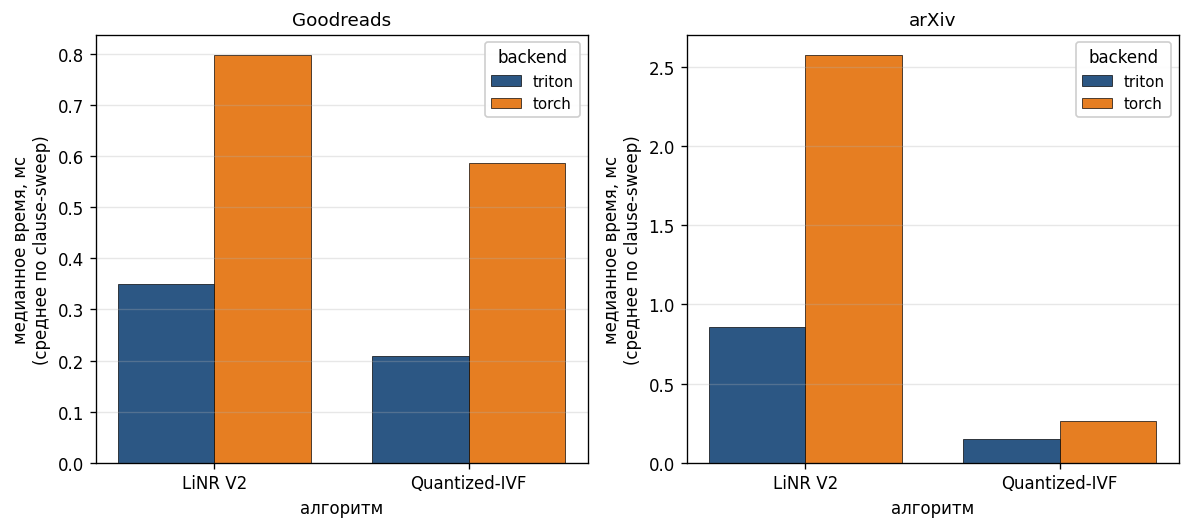
\includegraphics[width=\linewidth]{fig-4-1-backend-speedup.png}

\column{0.36\textwidth}
  \textbf{Анализ результатов}
  \begin{itemize}\footnotesize
    \item Медианное ускорение Triton-реализации
          по сравнению с эталонной на PyTorch
    \item PyTorch-бэкенд --- эталон для верификации корректности
  \end{itemize}

  \vspace{0.4em}
  \footnotesize Бэкенды переключаются параметром
  \texttt{backend="triton"/"pytorch"} без перекомпиляции графа.
\end{columns}
\end{frame}

% ── 12. МЕТОДОЛОГИЯ ЗАМЕРОВ ─────────────────────────────────────────────────
\begin{frame}
\frametitle{Методология замеров}

\begin{columns}[T]
\column{0.48\textwidth}
  \textbf{Метрики и эталоны}
  \begin{itemize}\footnotesize
    \item $\mathrm{Recall@}K(q) = |R_q\cap G_q|/\min(K,|G_q|)$
    \item С фильтрацией: эталон --- точный KNN с фильтром
    \item Без фильтрации: эталон --- реальные взаимодействия
    \item Время работы: медиана $t_\mathrm{med}$ по $4096$ батчам
    \item Память: размер индекса + \texttt{max\_memory\_allocated}
  \end{itemize}

  \vspace{0.3em}
  \textbf{Сетка экспериментов}
  \begin{itemize}\footnotesize
    \item Размерность: $d\in\{64,128,256\}$
    \item $K\in\{100,200,400,500,1000\}$
    \item Батч: $B\in\{1,8,16\}$
  \end{itemize}

\column{0.48\textwidth}
  \textbf{Аппаратный стенд}
  \begin{itemize}\footnotesize
    \item NVIDIA A100-SXM4-80GB
    \item Изолированный сервер, без сторонних задач во время замеров
  \end{itemize}

  \vspace{0.3em}
  \textbf{Изоляция}
  \begin{itemize}\footnotesize
    \item Каждая конфигурация --- отдельный Python-процесс
    \item $N_\mathrm{warmup}=20$ итераций прогрева перед каждым замером
    \item Замеры времени через \texttt{triton.testing.do\_bench}
    \item Компиляция: \texttt{torch.compile} в режиме
          \texttt{reduce-overhead}, \texttt{dynamic=True}
  \end{itemize}
\end{columns}
\end{frame}

% ── 13. НАБОРЫ ДАННЫХ И АТРИБУТЫ ─────────────────────────────────────────────
\begin{frame}
\frametitle{Наборы данных и атрибуты}

\begin{columns}[T]
\column{0.55\textwidth}
  \textbf{Наборы данных}
  \vspace{0.2em}

  {\footnotesize
  \begin{tabular}{lrrl}
    \toprule
    Набор & Объектов & Запросов & Энкодер \\
    \midrule
    Goodreads   & $797$\,K   & $313$\,K & gSASRec \\
    arXiv       & $2{,}99$\,M & $10$\,K  & Nomic-Embed \\
    Yambda-500M & $3{,}06$\,M & $46$\,K  & gSASRec \\
    Yambda-5B   & $5{,}37$\,M & $459$\,K & gSASRec \\
    \bottomrule
  \end{tabular}}

\column{0.42\textwidth}
  \textbf{Условия фильтрации} (Goodreads/arXiv)
  \begin{itemize}\footnotesize
    \item \textbf{C0--C3} --- одиночные атрибуты:\\
          Goodreads: жанр, язык, формат, год;\\
          arXiv: категория, лицензия, год, число версий
    \item \textbf{C4} --- пара атрибутов (жанр+язык / категория+год)
    \item \textbf{C5} --- объединение всех четырёх (наиболее строгое)
  \end{itemize}

  \vspace{0.4em}
  \textbf{Селективность условий:}\\
  C0 на arXiv: $\approx 5$--$30\%$ каталога;\\
  C5: $\lesssim 5\%$ --- крайне строгий фильтр.
\end{columns}
\end{frame}

% ── 14. РЕЗУЛЬТАТЫ БЕЗ ФИЛЬТРАЦИИ ────────────────────────────────────────────
\begin{frame}
\frametitle{Результаты: поиск без фильтрации и потребление памяти}

\begin{columns}[c]
\column{0.54\textwidth}
  \centering
  {\scriptsize
  \setlength{\tabcolsep}{4pt}
  \begin{tabular}{lcccc}
    \toprule
    Набор (Recall@100) & LiNR V1 & LiNR V4 & LiNR V3 & QuantizedIVF \\
    \midrule
    Goodreads     & $0{,}1479$ & $0{,}1478$ & $0{,}1438$ & $0{,}1449$ \\
    Yambda-500M   & $0{,}1486$ & $0{,}1485$ & $0{,}1426$ & $0{,}1468$ \\
    Yambda-5B     & $0{,}1779$ & $0{,}1778$ & $0{,}1590$ & $0{,}1739$ \\
    \bottomrule
  \end{tabular}}\\[0.5em]
  {\footnotesize \textbf{Recall@100}, $d=128$, $B=1$, Triton, эталон --- реальные взаимодействия пользователей.}

\column{0.44\textwidth}
  \centering
  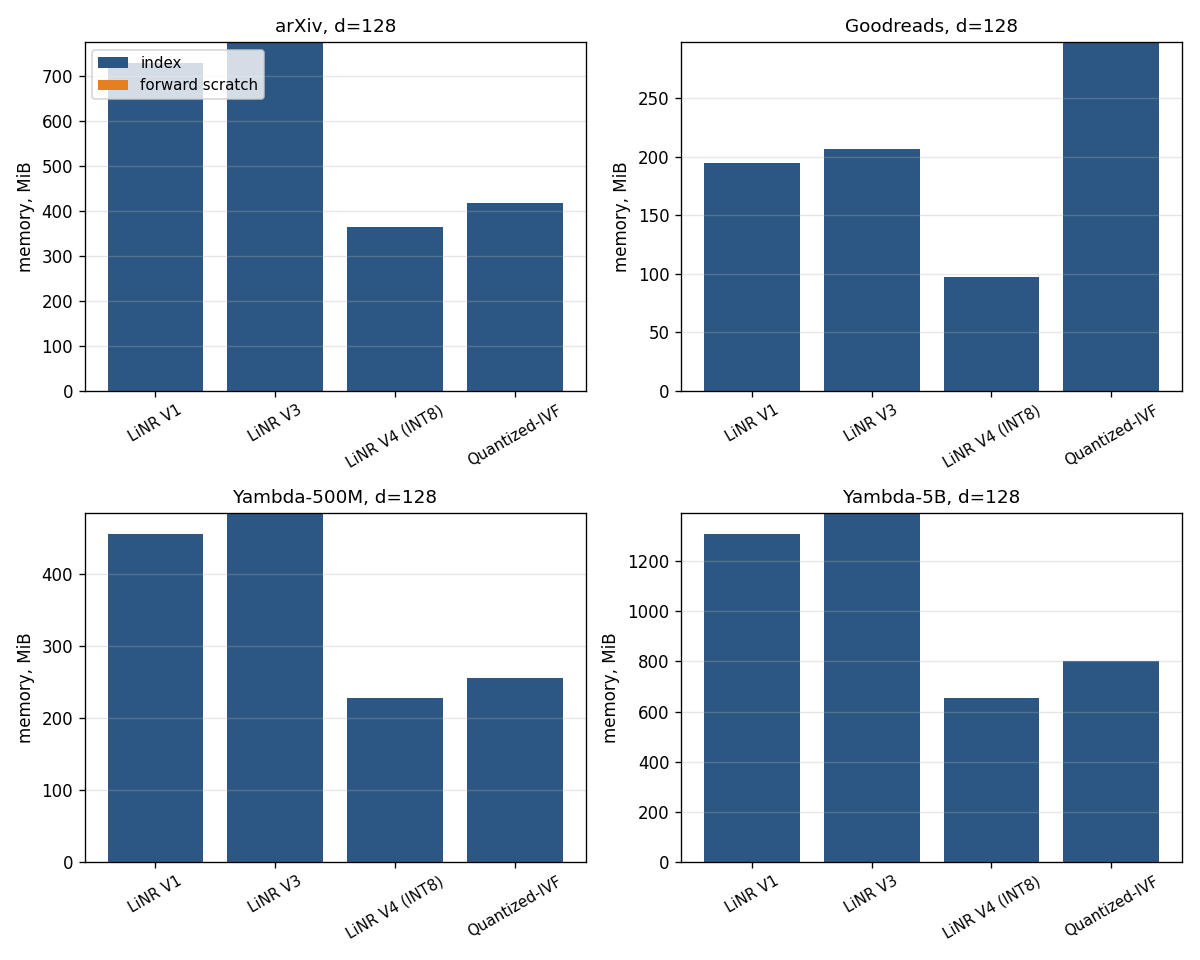
\includegraphics[height=0.73\textheight,keepaspectratio]{fig-6-4-memory-per-algo.png}\\
  {\footnotesize Объем памяти индекса ($d=128$).}
\end{columns}
\end{frame}

% ── 15. ПАРЕТО С ФИЛЬТРАЦИЕЙ ─────────────────────────────────────────────────
\begin{frame}
\frametitle{Результаты: Парето-фронт качества, скорости и памяти (arXiv)}

\begin{columns}[T]
\column{0.55\textwidth}
  \centering
  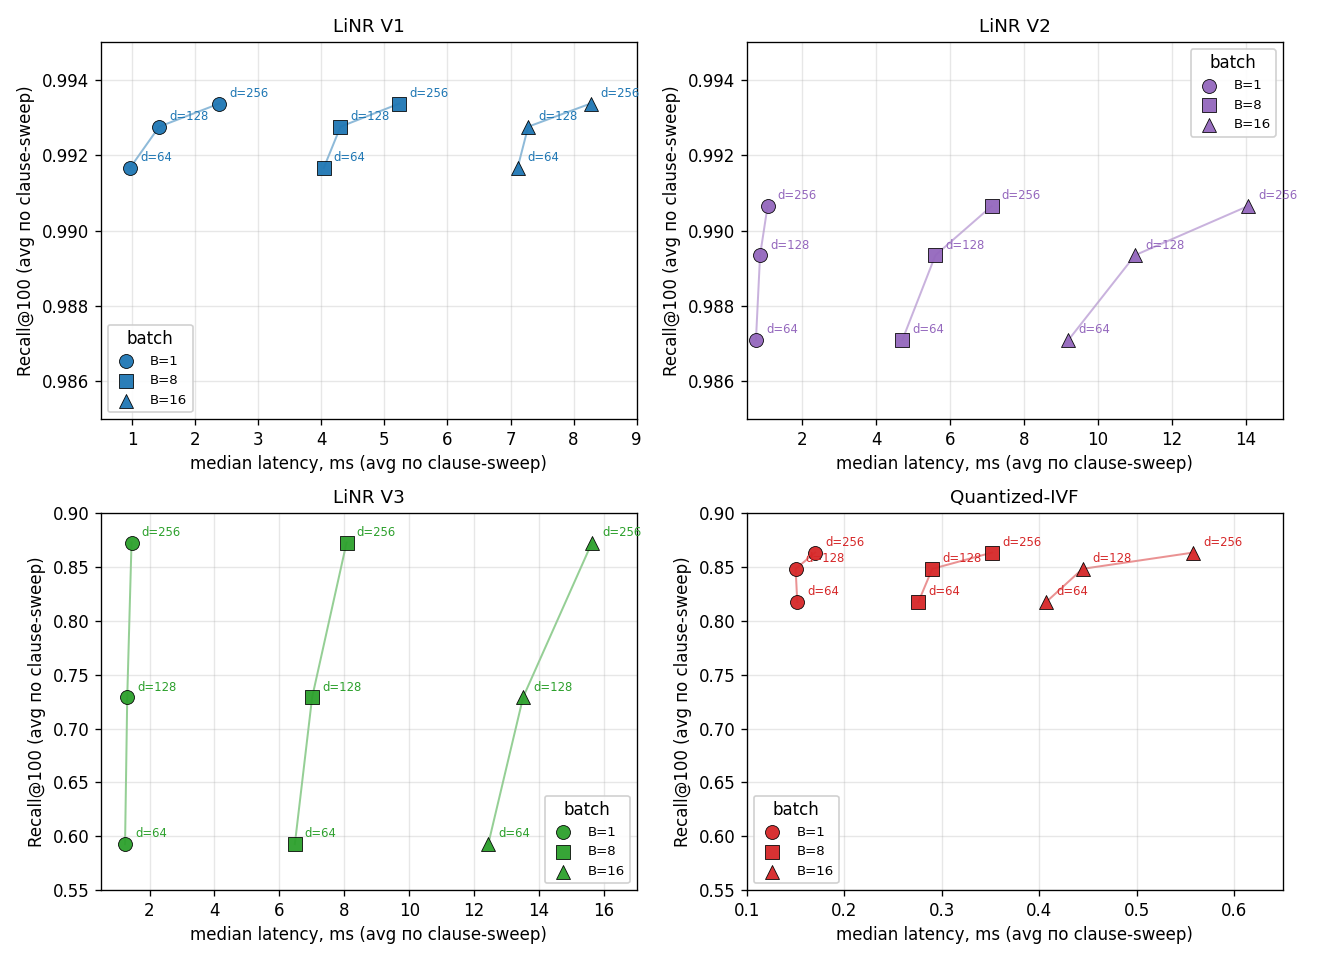
\includegraphics[width=\linewidth]{fig-6-1-pareto-quality-latency.png}\\
  {\footnotesize arXiv, $d=128$, $K=100$, $B=1$.}

\column{0.43\textwidth}
  {\footnotesize Полнота, ускорение и память; $d=128$, $K=100$, $B=1$.}\\[0.3em]
  {\footnotesize
  \textbf{arXiv}\\[0.15em]
  \begin{tabular}{llccc}
    \toprule
    Усл. & Алгоритм & Recall & Уск. & МиБ \\
    \midrule
    \textbf{C0} & LiNR V1       & $0{,}99$ & $1{,}00\times$ & $730$ \\
        & LiNR V2       & $0{,}99$ & $1{,}68\times$ & $730$ \\
        & LiNR V4       & $0{,}95$ & $0{,}70\times$ & $365$ \\
        & LiNR V3       & $0{,}68$ & $1{,}08\times$ & $775$ \\
        & \alert{QuantizedIVF} & $0{,}88$ & $\mathbf{9{,}40\times}$ & $419$ \\
    \midrule
    \textbf{C5} & LiNR V2       & $0{,}99$ & $1{,}76\times$ & $730$ \\
        & LiNR V3       & $0{,}92$ & $1{,}10\times$ & $775$ \\
        & \alert{QuantizedIVF} & $0{,}76$ & $\mathbf{9{,}47\times}$ & $427$ \\
    \bottomrule
  \end{tabular}\\[0.5em]

  \textbf{Goodreads} (C0)\\[0.15em]
  \begin{tabular}{lccc}
    \toprule
    Алгоритм & Recall & Уск. & МиБ \\
    \midrule
    LiNR V1       & $1{,}00$ & $1{,}00\times$ & $195$ \\
    LiNR V2       & $0{,}99$ & $1{,}33\times$ & $195$ \\
    LiNR V4       & $0{,}96$ & $0{,}74\times$ & $97$ \\
    LiNR V3       & $0{,}75$ & $1{,}18\times$ & $207$ \\
    \alert{QuantizedIVF} & $0{,}91$ & $\mathbf{2{,}19\times}$ & $298$ \\
    \bottomrule
  \end{tabular}}
\end{columns}
\end{frame}

% ── 16. СЕЛЕКТИВНОСТЬ ────────────────────────────────────────────────────────
\begin{frame}
\frametitle{Устойчивость алгоритмов к селективности фильтра}

\begin{center}
  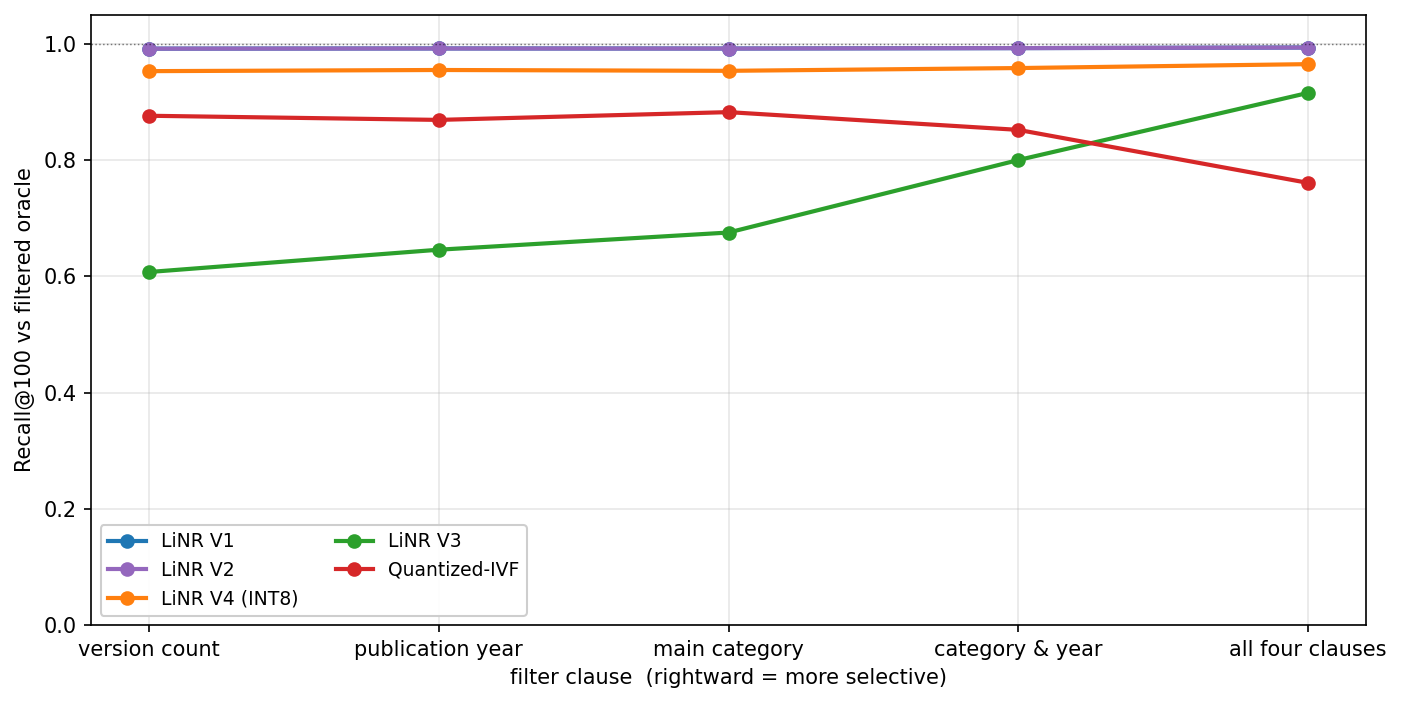
\includegraphics[height=0.72\textheight,keepaspectratio]{fig-6-5-selectivity-recall.png}\\[0.4em]
  {\footnotesize Recall@100 в зависимости от селективности условия на arXiv
  ($d=128$, $K=100$, $B=1$).}
\end{center}
\end{frame}

% ── 17. МАСШТАБИРУЕМОСТЬ: размер батча ─────────────────────────────────────────
\begin{frame}
\frametitle{Масштабируемость алгоритмов}

\begin{center}
  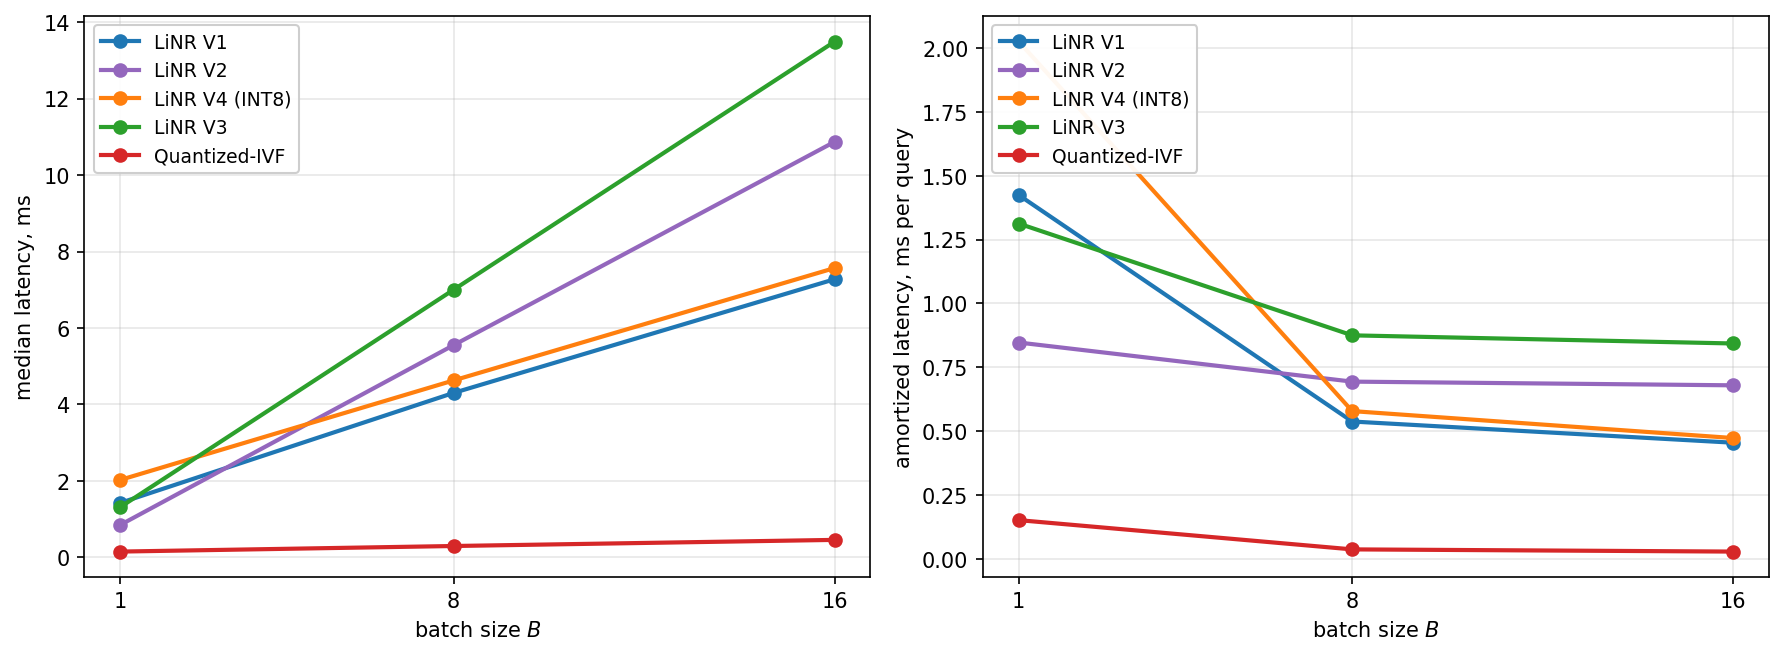
\includegraphics[height=0.74\textheight,keepaspectratio]{fig-6-3-batch-scaling.png}\\[0.4em]
  {\footnotesize Амортизированное время (мс/запрос) от размера батча $B$ (arXiv, $d=128$, $K=100$).}
\end{center}
\end{frame}

% ── 17b. МАСШТАБИРУЕМОСТЬ: размерность ─────────────────────────────────────────
\begin{frame}
\frametitle{Зависимость скорости от размерности эмбеддингов}

\begin{center}
  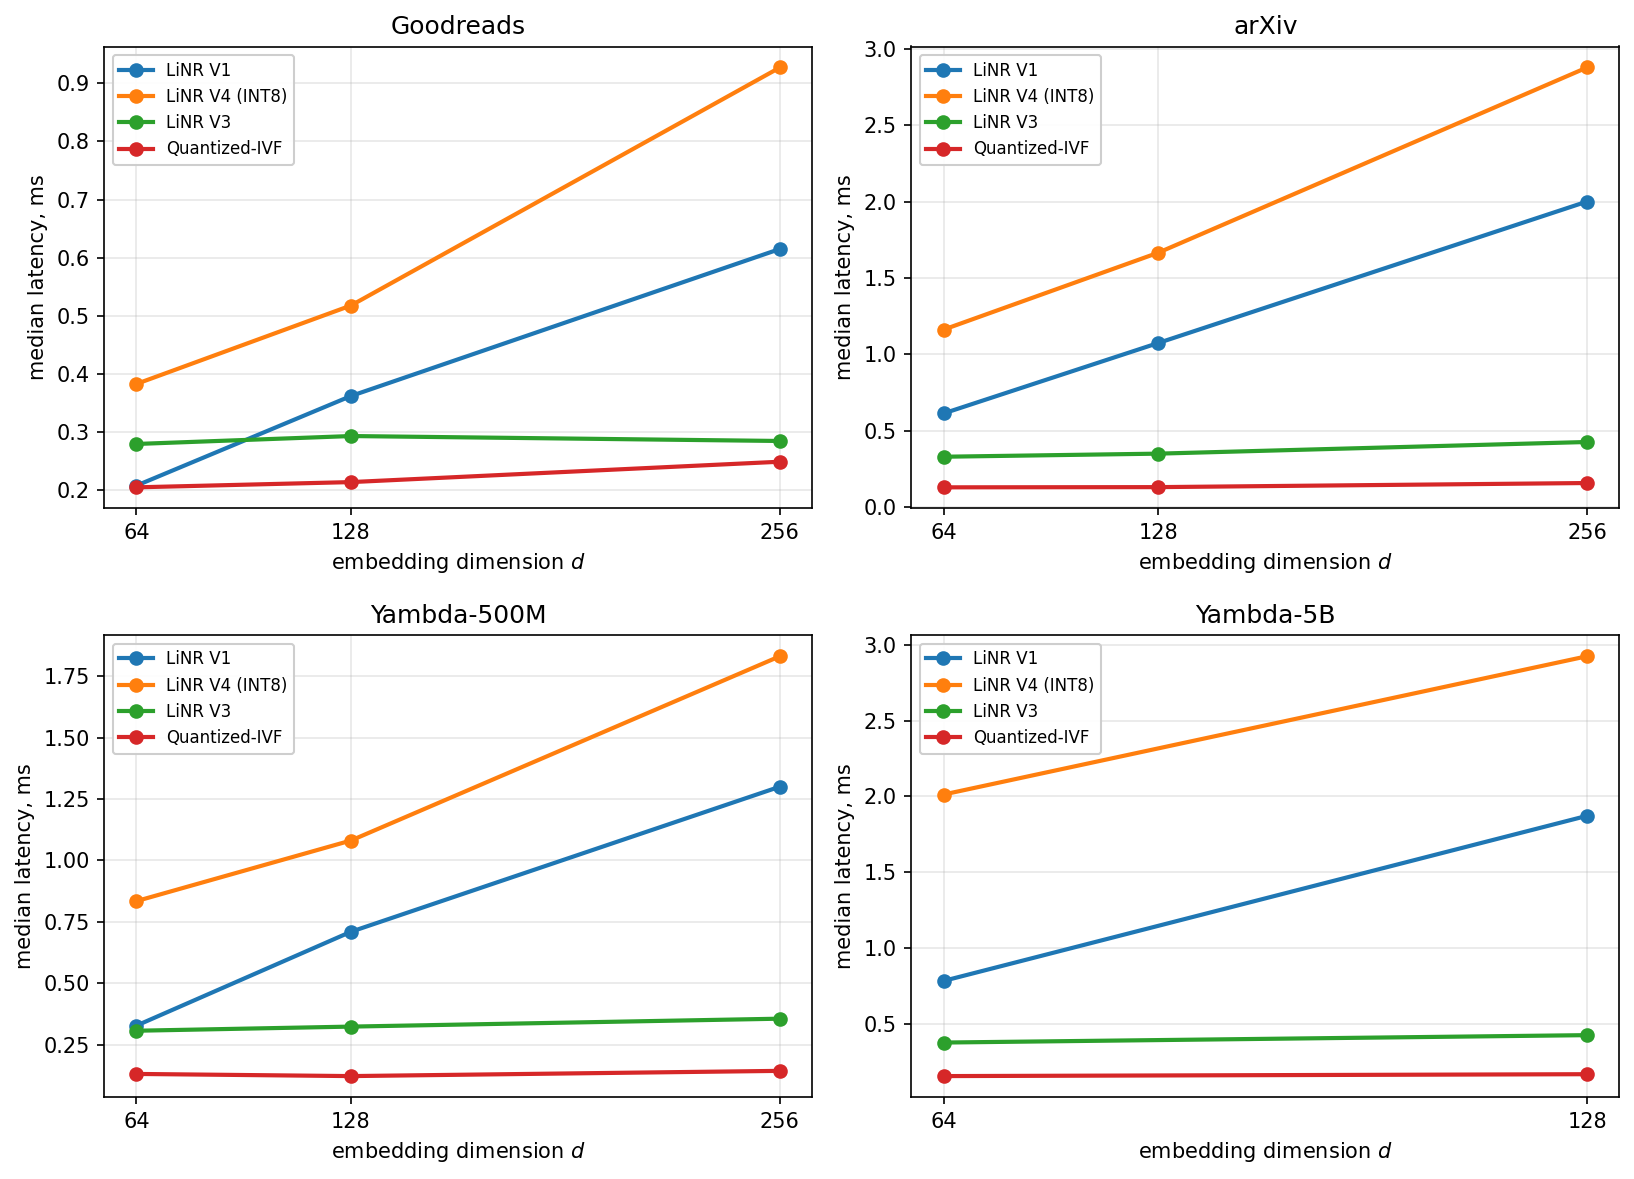
\includegraphics[width=0.9\linewidth,trim={0 283 0 0},clip]{fig-6-9-dim-scaling.png}\\[0.4em]
  {\footnotesize Зависимость скорости алгоритмов от размерности векторов $d$.}
\end{center}
\end{frame}

% ── 18. АППАРАТНЫЕ ОСОБЕННОСТИ ─────────────────────────────────────────────────
\begin{frame}
\frametitle{Чувствительность к гиперпараметрам алгоритма QuantizedIVF}

\begin{center}
  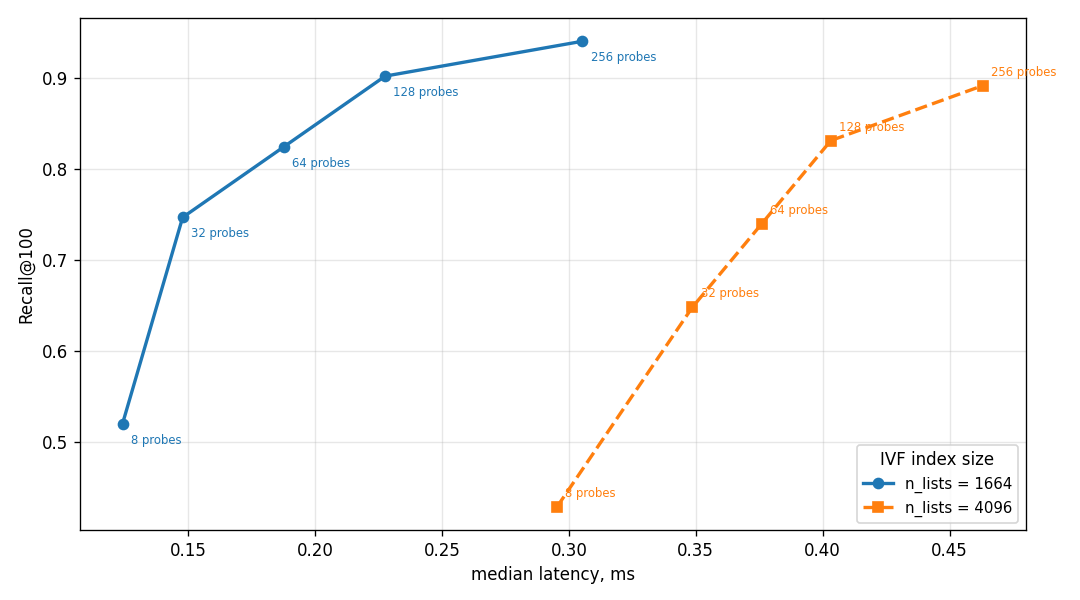
\includegraphics[height=0.72\textheight,keepaspectratio]{fig-6-7-silvertorch-pareto.png}\\[0.4em]
  {\footnotesize Парето-кривые QuantizedIVF при разном числе кластеров $n_\mathrm{lists}$ (arXiv, \textbf{C5}).}
\end{center}
\end{frame}

% ── 19. ЗАКЛЮЧЕНИЕ ───────────────────────────────────────────────────────────
\begin{frame}
\frametitle{Заключение}

\textbf{Результаты работы}
\begin{enumerate}
  \item \textbf{QuantizedIVF} --- ускорение до ${\approx}9\times$
        при полноте $76$--$94\%$. Компактный индекс и гибкость делают его оптимальным выбором по умолчанию
        для крупных каталогов.
  \item \textbf{LiNR V2} --- оптимальный выбор при строгих фильтрах:
        полнота близка к идеальной, решает проблему нехватки кандидатов.
  \item \textbf{LiNR V4} --- размер индекса в два раза меньше при Recall $\ge 95\%$;
        при размере батча $B=16$ время работы сравнивается с V1.
  \item Фреймворк \texttt{torchretrieve} и все эксперименты опубликованы в открытом доступе ---
        решена проблема воспроизводимости промышленных методов.
\end{enumerate}

\vspace{0.4em}
\textbf{Направления дальнейшей работы}
\begin{itemize}\small
  \item Шардирование каталога между несколькими GPU (multi-GPU sharding)
  \item Потоковое обновление индекса в реальном времени
\end{itemize}
\end{frame}

% ── 20. СПАСИБО ──────────────────────────────────────────────────────────────
\begin{frame}[plain]
\begin{center}
  \vfill
  {\LARGE\textit{Спасибо за внимание!}}
  \vfill
\end{center}
\end{frame}

\end{document}
